\section{Theory}
\subsection{Basic theory of grating spectrometer}

\subsection{Optical Fiber / brewster angle}

\subsubsection{Blackbody radiation}
All matter emits electromagnetic radiation when it has a temperature above absolute zero. This radiative distribution of entropy is called thermal radiation and is a spontaneous process.

Similarly, all matter absorbs electromagnetic radiation to some degree. In addition, a blackbody is an object that absorbs all radiation of all wavelengths that falls upon it. Furthermore, at thermal equillibrium a blackbody emits a characteristic frequency distribution, which is temperature depended.


\subsection{Light bulbs and the solar spectrum}

\begin{figure}[h!]
    \centering
    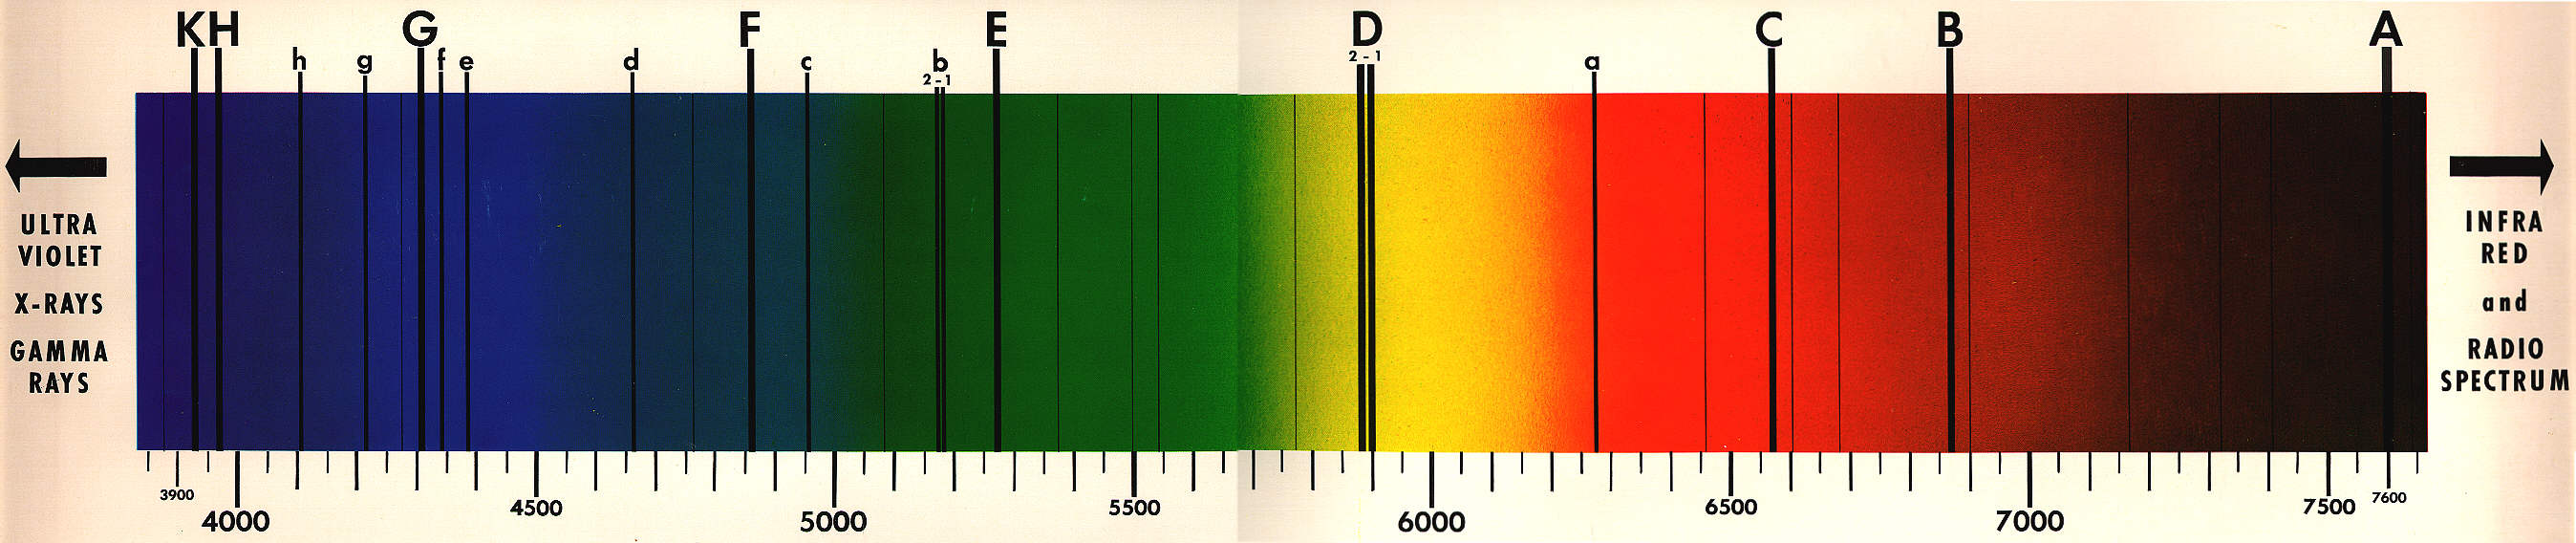
\includegraphics[width=0.5\textwidth]{solarspectrum}
    \caption{The solar spectrum}
    \label{fig:solarspectrum}
\end{figure}

Wiens displacement law

\begin{equation}
    \lambda_{\text{peak}}T = & \SI{2.898e-3}{\meter\kelvin} \label{eq:wien}
\end{equation}
